\documentclass{article}
\usepackage[brazil]{babel}
\usepackage[utf8]{inputenc}
\usepackage[T1]{fontenc}% optional T1 font encoding
\usepackage[%
    colorlinks=true,
    pdfborder={0 0 0},
    linkcolor=red
]{hyperref}
\usepackage[all]{hypcap}
\usepackage{amsmath}
\interdisplaylinepenalty=2500
\usepackage{graphicx}
\usepackage[cmintegrals]{newtxmath}
\usepackage{cite}
\usepackage{listings}
\usepackage{hyperref}
\usepackage{indentfirst}
\usepackage{siunitx}
\usepackage{textgreek}
\usepackage[portuguese,linesnumbered,ruled]{algorithm2e}
\usepackage{multirow}
\usepackage{anysize}

\begin{document}

    \title{Preparação do Exp. IV — Estágio de acoplamento com Transistor de Junção Bipolar (BJT)}
    \author{Bianca Yoshie Itiroko - 164923, Luiz Eduardo Cartolano - 183012, Seong Eun Kim - 177143 \\ EE534 - Turma Y - Grupo 2}
    \date{Setembro de 2018}

    \maketitle

    \section{Topologia do circuito} \label{sec:1}
        Considerando os seguintes requisitos:
        \begin{itemize}
            \item Alto ganho de corrente;
            \item Ganho de tensão $=$ 1;
            \item Resistência de entrada alta;
            \item Resistência de saída baixa.
        \end{itemize}
        Podemos concluir que o \emph{BJT} deve ser usado com a topologia de \textbf{\emph{Coletor comum (Seguidor de Emissor)}}. A escolha por tal topologia se da com base nas equações apresentadas no \cite{Sedra2004}. Para um circuito desse tipo (Figura \ref{fig:coletor}), podemos chegar nas seguintes equações para os parâmetros (usa-se o circuito equivalente para pequenos sinais, Figura \ref{fig:eq_coletor} a fim de facilitar encontrar as equações):
        \begin{itemize}
            \item Ganho de tensão
                \begin{equation}
                    A_v = \frac{(\beta + 1) \cdot R_L \parallel r_o}{R_s + (\beta + 1) \cdot (r_e + R_L \parallel r_o) }
                \end{equation}
            \item Impedância de entrada
                \begin{equation}
                    R_i = (\beta + 1) \cdot R_L
                \end{equation}
            \item Impedância de saída
                \begin{equation}
                    R_o = \frac{r_\pi + R_s}{\beta + 1}
                \end{equation}
            \item Corrente no terminal de saída
                \begin{equation}
                    i_x = v_x \cdot [\frac{1}{r_o} + \frac{\beta + 1}{r_\pi + R_s}]
                \end{equation}
        \end{itemize}
        
        Analisando as equações, é possível perceber que o circuito em questão atende aos requisitos, por isso é uma boa escolha.
        
    \section{Projeto de um amplificador como estágio de acoplamento}
        \subsection{a) Valor de V$_{CE}$ de modo que se obtenha a máxima excursão}
            O ponto de máxima excursão para o transistor visa obter o seu funcionamento, a maior parte do tempo, em modo linear. Para encontrá-lo é preciso que a tensão no emissor, V$_E$, esteja a meio caminho entre a tensão limiar de funcionamento, V$_{BE}$ e a tensão de alimentação, V$_{CC}$. Para isso fazemos:
            \begin{equation}
                V_E = \frac{V_{BE} + V_{CC}}{2}
            \end{equation}
            Para o qual encontramos V$_E$ = 6,35V. Sabendo que:
            \begin{equation}
                V_B = V_{BE} + V_E
            \end{equation}
            Temos que V$_B$ = 7,05V. E, uma vez que V$_{C} = V_{CC}$ = 12V e que:
            \begin{equation}
                V_{CE} = V_C - V_E
            \end{equation}
            Podemos concluir que V$_{CE}$ = 5,65V.
        
        \subsection{b) Calcule o ganho, impedância de entrada e impedância de saída para pequenos sinais}
            Primeiro, iremos mostrar o cálculo para a impedância de entrada. Analisando o circuito equivalente da Figura \ref{fig:eq_coletor}, podemos perceber que a resistência efetiva no emissor é dada por $r_e + R_E$. Logo, a impedância no transistor é $Z_{in} = (r_e + R_E) \cdot \beta $. E então, é possível concluir que a impedância de entrada do circuito vai ser aproximadamente igual ao resistor $R_B$.
            
            Já para calcularmos a impedância de saída, a abordagem foi semelhante. Sobre o mesmo circuito usado anteriormente, aplicou-se Thévenin, de onde obtemos que $Z_{TH} = R_g \parallel R_B$, e $V_{TH} = V_B$. Analisando a tensão de saída, foi possível perceber que $R_E$ está em paralelo com a tensão de saída do transistor, logo:
            \begin{equation}
                Z_{o}(T) = \frac{R_g \parallel R_B}{\beta} + r_e
            \end{equation}
            E como $R_E$ é muito maior que $Z_{o}(T)$, a impedância de saída será, aproximadamente, a impedância de saída do transistor, logo:
            \begin{equation}
                Z_o = r_e = \frac{\beta}{\beta + 1} \cdot \frac{V_T}{I_C}
            \end{equation}
            Que é um valor extremamente baixo.
            
            Por fim, buscou-se descobrir o ganho de tensão($A_v$) do circuito. Para isso comparou-se a tensão de entrada com a de saída, obtendo:
            \begin{equation}
                A_v = \frac{R_E \cdot i_e}{(R_E \cdot i_e) + r_e}
            \end{equation}
            Como, $R_E$ é muito maior que $r_e$, o ganho de tensão pode ser considerado igual a 1.
            
         \subsection{c) Encontre o valor de R$_E$ x I$_C$}
            Sabemos que:
            \begin{equation}
                i_c = (\frac{\beta}{\beta + 1}) \cdot i_e
            \end{equation}
            Uma vez que, analisando o circuito em \cite{ref:roteiro}, encontramos:
            \begin{equation}
                i_e = \frac{V_E}{R_E}
            \end{equation}
            Foi possível obter que $i_c \cdot R_E = 6,29$.
            
         \subsection{d) Encontre o valor de R$_B$ x I$_C$}
            Uma vez que, analisando o circuito em \cite{ref:roteiro}, encontramos:
            \begin{equation}
                i_b = \frac{V_{CC} - V_B}{R_B}
            \end{equation}
            E sabendo que:
            \begin{equation}
                i_c = \beta \cdot i_b
            \end{equation}
            Foi possível obter que $i_c \cdot R_B = 594$.
            
         \subsection{e) Encontre o valor de R$_B$ \textbackslash R$_E$}
            Sabemos que:
            \begin{equation}
                i_b = \frac{i_e}{\beta + 1}
            \end{equation}
            Uma vez que, analisando o circuito em \cite{ref:roteiro}, encontramos:
            \begin{equation}
                \frac{V_{CC} - V_{B}}{R_B} = \frac{V_E}{R_E \cdot (\beta + 1)}
            \end{equation}
            Foi possível obter que R$_B$ \textbackslash R$_E$ = 94,3.        
            
        \subsection{f) Encontre R$_B$ e R$_E$ para I$_C$ = I$_{C,máx \textbackslash 2}$ e para I$_C$ =100mA. Extraia I$_{C,máx}$ do datasheet.}
            A partir do \emph{datasheet} \citeonline{ref:datasheet}, foi possível descobrir que $I_{C,max} = 600 mA$. 
            
            Então usando as equações obtidas nos itens anteriores, obtemos que, para $I_C = $ I$_{C,máx \textbackslash 2}$ = 300mA, \textbf{R$_E = 20\Omega$} e \textbf{R$_B = 2k\Omega$}.
            
            Enquanto que para $I_C = 100mA$, \textbf{R$_E = 62,5\Omega$} e \textbf{R$_B = 6k\Omega$}.
        
        \subsection{g) Para os valores encontrados no item anterior de R$_B$ e R$_E$ para I$_C$ =100mA, calcule os valores numéricos do ganho, impedância de entrada e impedância de saída. Assuma V$_T$ = 26mV. Comente estes valores sob a perspectiva do item 1.}
            Usando as equações e as discussões dos itens anteriores, podemos concluir que:
            \begin{itemize}
                \item Impedância de entrada = 6 k$\Omega$
                \item Impedância de saída = 0,25 $\Omega$
                \item Ganho de tensão = 1V
            \end{itemize}
            
            Os valores encontrados vão ao encontro do que discutimos no Item \ref{sec:1}. O circuito simulado com os valores das resistências calculadas pode ser visto em \citeonline{ref:simu}.
        
    \nocite{*}
    \bibliographystyle{plain}
    \bibliography{references}

    \begin{figure}[!h]
        \centering
        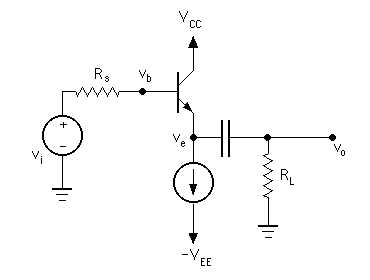
\includegraphics{cc_amp_1.jpg}
        \caption{Exemplo de circuito para o Coletor Comum}
        \label{fig:coletor}
    \end{figure}
    
    \begin{figure}[!h]
        \centering
        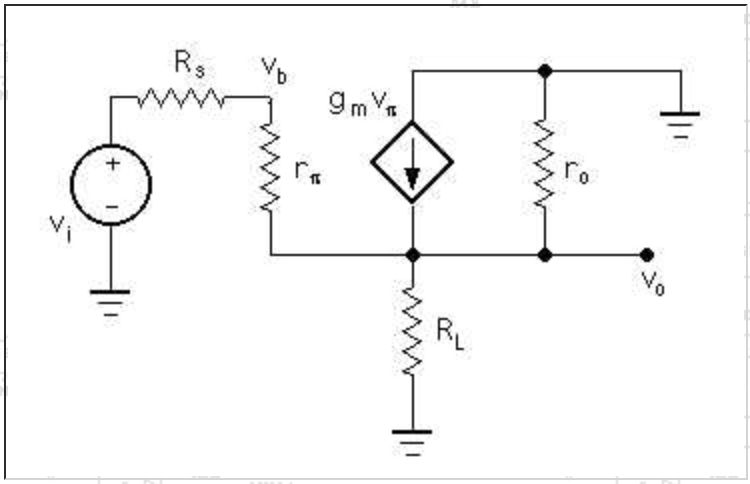
\includegraphics{coletorcomum.png}
        \caption{Exemplo de circuito equivalente de pequenos sinais para o Coletor Comum}
        \label{fig:eq_coletor}
    \end{figure}


\end{document}

